\section{Maß}
	Das Ergebnis einer Lebegueschen Integration kann ganz allgemein als $n$-dimensionales Maß betrachtet werden. Abhängig von der Dimension kann es sich dabei um eine Strecke, Fläche, Volumen oder abstraktere Formen handeln. Um eine Intuition zu vermitteln soll in diesem Abschnitt sehr knapp die Lebeguesche Maßtheorie eingeführt werden.
	
	\subsection{Motivation}
	Volumenberechnung, Flächenberechnung, Dichtenberechnung.
	
	\subsection{d-dimesionales Volumen}
	Gegeben sei ein Quader $Q \subset \R^d$. Dies lässt sich beschreiben als die Menge
	\begin{equation}
		Q = \lbrace (x_1, ..., x_d\|a_i \leq x_i \leq b_i \| i = 1, ..., d \rbrace  \subset \R^d
	\end{equation}
	Dabei gilt $-\infty <a_i \leq b_i < \infty$ und jedes $\leq$ darf durch $<$ ersetzt werden. Das Volumen dieses Quaders ist nun gegeben durch
	\begin{equation}
		v_d(Q) = \prod_{i=1}^d (b_i - a_i) \qquad \in \R
	\end{equation}
	Wichtig hierbei ist der Unterschied des im Sprachgebrauch bekannten Volumen (bekanntermaßen im $R^3$) und dem hier verwendeten Volumen, dass dem Maß der jeweiligen Dimension entspricht.
	Zur Bestimmung des Volumens einer beliebigen Menge pflastert man diese gedanklich mit mehreren der bereits bekannten Quadern und erhält 
	\begin{equation}
		v_d(E) = \inf \sum_{k = 1}^\infty v_d (Q_k)
	\end{equation}
	wobei $(Q_k)$ eine beliebige Folge von Quadern $Q_k \subset \R^d$ ist. Dabei muss gelten:
	\begin{equation}
		E \subset \bigcup_{k=1}^\infty Q_k
	\end{equation}
	  \begin{figure}[H] 
		  \centering
		  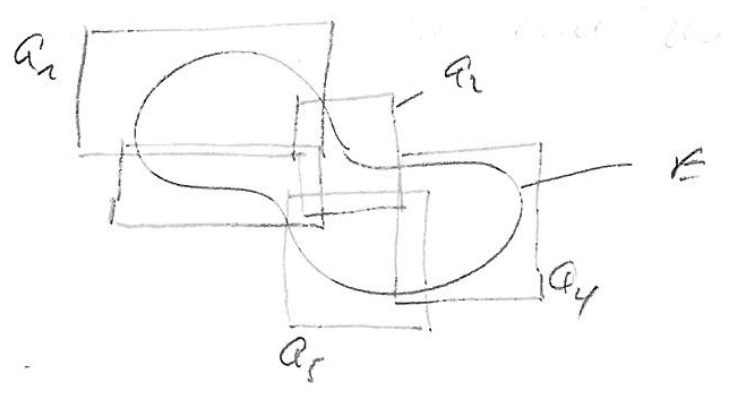
\includegraphics[width=0.5\textwidth]{./img/mass_dvol_a.png}
		  \caption{Rasterung \protect\cite{HM3}}
		  \label{fig:rasterung}
	  \end{figure}
	  
	  \subsection{Elementarfunktionen}
	  Eine Funktion $s: \R^d \rightarrow \R$ die nur endlich viele Werte $\alpha_1, ..., \alpha_n \in \R$ annimmt heißt Elementar- oder auch Treppenfunktion.
	  Setzt man
	  \begin{equation}
	  	A_k := \lbrace x \in \R^d \| s(x) = x_k\rbrace
	  \end{equation}
	  dann gilt 
	  \begin{equation}
	  	s = \sum_{k=1}^n\alpha_k \textsl{x}_{A_k}
	  \end{equation}
	  
	  \begin{satz} \label{th:leb_elem_folg}
	  	Zu jeder Funktion $f \geq 0$ gibt es eine Folge von Elementarfunktionen $s_n\;, n \in \N$ mit
	  	\begin{align*}
	  		0 \leq s_n \leq s_{n+1} \leq ... \leq f \\
	  		\lim_{n \to \infty} s_n(x) = f(x) 
	  	\end{align*}
	  	Man kürzt ab mit 
	  	$s_n(x) \nearrow f(x) \; (n \rightarrow \infty)$.
	  \end{satz}
	  \begin{figure}[H] 
		  \centering
		  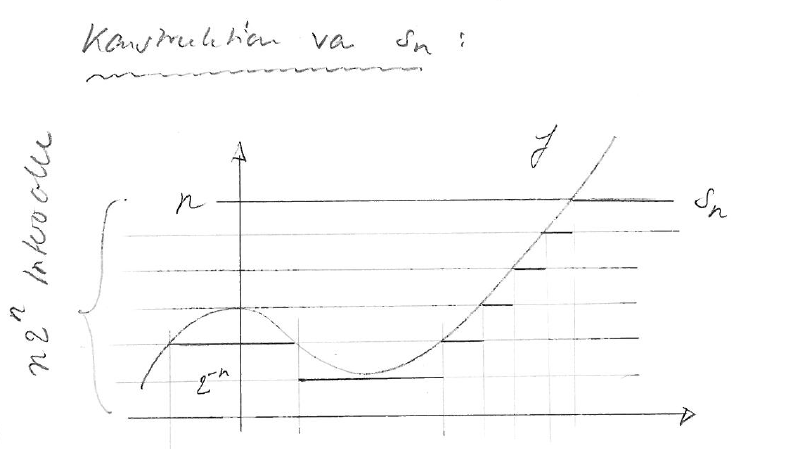
\includegraphics[width=0.5\textwidth]{./img/mass_treppf.png}
		  \caption{Treppenfunktion \protect\cite{HM3}}
		  \label{fig:treppenf}
	  \end{figure}